\documentclass[tikz,border=0pt,11pt]{standalone}
\usepackage[T1]{fontenc}
\usepackage[utf8]{inputenc}
\usepackage{lmodern,amsmath,amssymb}
\usepackage[swedish]{babel}
\usetikzlibrary{arrows.meta,calc,positioning,decorations.pathmorphing,decorations.pathreplacing,patterns,shadings}
\definecolor{navy}{HTML}{102F40}
\definecolor{teal}{HTML}{147D78}
\definecolor{lightteal}{HTML}{E6F1ED}
\definecolor{gold}{HTML}{B88B3B}
\definecolor{palegold}{HTML}{F7EEDB}
\definecolor{rust}{HTML}{B6533B}
\definecolor{palerust}{HTML}{FAEAE4}
\definecolor{paper}{HTML}{F7F5EE}
\definecolor{muted}{HTML}{5B6D72}
\definecolor{line}{HTML}{D6DED8}
\renewcommand{\familydefault}{\sfdefault}
\newcommand{\atom}[5]{\shade[ball color=#3!70] (#1,#2) circle (#5);\node[text=white,font=\bfseries\small] at (#1,#2){#4};}
\newcommand{\water}[3]{\begin{scope}[shift={(#1,#2)},scale=#3]\draw[navy!45,line width=2pt] (-.3,.22)--(0,0)--(.3,.22);\atom{0}{0}{rust}{O}{.22}\atom{-.3}{.22}{teal}{H}{.15}\atom{.3}{.22}{teal}{H}{.15}\end{scope}}
\newcommand{\panel}[4]{\filldraw[fill=white,draw=line,rounded corners=5pt] (#1,#2) rectangle ++(#3,#4);}
\newcommand{\note}[4]{\node[txt,text width=#3cm] at (#1,#2){#4};}
\tikzset{txt/.style={anchor=north west,align=left,text=navy,font=\small},
 head/.style={anchor=west,text=navy,font=\bfseries\large},
 label/.style={align=center,text=navy,font=\small},
 smalllabel/.style={align=center,text=muted,font=\footnotesize},
 arrow/.style={-{Latex[length=2.5mm,width=1.8mm]},line width=1.2pt,draw=teal},
 goldarrow/.style={-{Latex[length=2.5mm]},line width=1.2pt,draw=gold},
 rustarrow/.style={-{Latex[length=2.5mm]},line width=1.2pt,draw=rust},
 dashedarrow/.style={arrow,dashed},
 badge/.style={fill=lightteal,rounded corners=3pt,text=teal,font=\bfseries\small,inner sep=5pt}}
\begin{document}
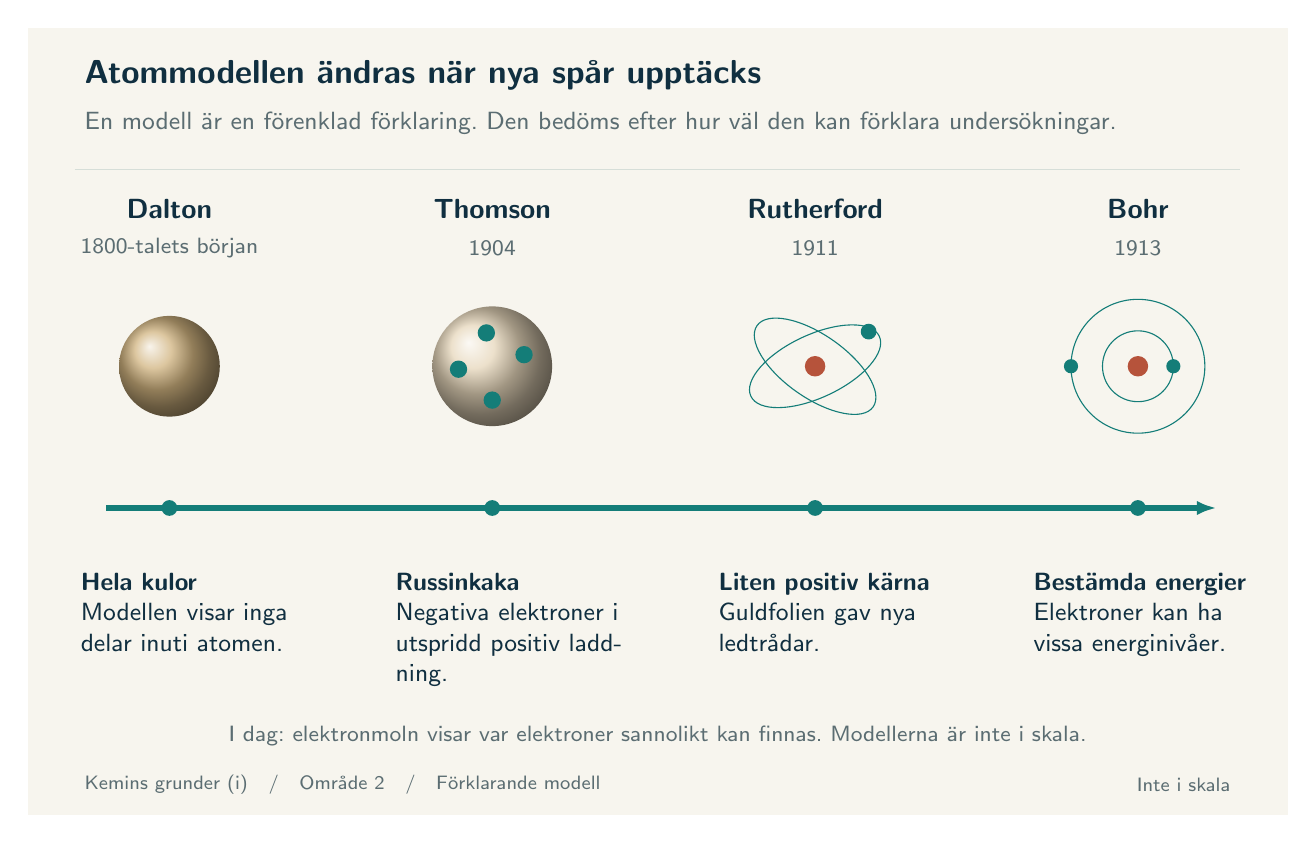
\begin{tikzpicture}[x=1cm,y=1cm]
\path[use as bounding box] (0,0) rectangle (16,10);
\fill[paper] (0,0) rectangle (16,10);
\node[head] at (.6,9.4){Atommodellen ändras när nya spår upptäcks};
\note{.6}{9.05}{14.8}{\textcolor{muted}{En modell är en förenklad förklaring. Den bedöms efter hur väl den kan förklara undersökningar.}}
\draw[line] (.6,8.2)--(15.4,8.2);

\draw[arrow,line width=2pt] (1,3.9)--(15.1,3.9);
\foreach \x/\name/\date in {1.8/Dalton/1800-talets början,5.9/Thomson/1904,10/Rutherford/1911,14.1/Bohr/1913}{\node[label,font=\bfseries] at (\x,7.7){\name};\node[smalllabel] at (\x,7.2){\date};\fill[teal] (\x,3.9) circle(.10);}
\shade[ball color=gold!65] (1.8,5.7) circle(.64);
\shade[ball color=gold!35] (5.9,5.7) circle(.76);\foreach \a in {20,100,185,270}{\fill[teal] ($(5.9,5.7)+(\a:.43)$) circle(.11);}
\fill[rust] (10,5.7) circle(.13);\draw[teal,rotate around={25:(10,5.7)}] (10,5.7) ellipse(.9 and .4);\draw[teal,rotate around={-35:(10,5.7)}] (10,5.7) ellipse(.9 and .4);\fill[teal] (10.68,6.14) circle(.1);
\fill[rust] (14.1,5.7) circle(.13);\draw[teal] (14.1,5.7) circle(.45);\draw[teal] (14.1,5.7) circle(.85);\fill[teal] (14.55,5.7) circle(.09);\fill[teal] (13.25,5.7) circle(.09);
\note{.55}{3.2}{3.0}{\textbf{Hela kulor}\par Modellen visar inga delar inuti atomen.}
\note{4.55}{3.2}{3.0}{\textbf{Russinkaka}\par Negativa elektroner i utspridd positiv laddning.}
\note{8.65}{3.2}{3.0}{\textbf{Liten positiv kärna}\par Guldfolien gav nya ledtrådar.}
\note{12.65}{3.2}{2.85}{\textbf{Bestämda energier}\par Elektroner kan ha vissa energinivåer.}
\node[smalllabel,text width=14.2cm] at (8,1.0){I dag: elektronmoln visar var elektroner sannolikt kan finnas. Modellerna är inte i skala.};\node[anchor=west,text=muted,font=\scriptsize] at (.6,.38){Kemins grunder (i)\quad /\quad Område 2\quad /\quad Förklarande modell};
\node[anchor=east,text=muted,font=\scriptsize] at (15.4,.38){Inte i skala};
\end{tikzpicture}\end{document}
